\documentclass[tikz,border=5pt]{standalone}
\usepackage[T1]{fontenc}
\usepackage{lmodern,amsmath,amssymb}
\usetikzlibrary{arrows.meta,calc,positioning,fit,backgrounds,shapes.geometric,matrix,decorations.pathreplacing,patterns}
\definecolor{ink}{gray}{0.08}
\definecolor{wash}{gray}{0.965}
\definecolor{soft}{gray}{0.45}
\tikzset{box/.style={draw=ink,line width=.65pt,fill=white,align=center,inner sep=4pt,outer sep=0pt,font=\small},flow/.style={draw=ink,line width=.65pt,-{Latex[length=1.8mm,width=1.3mm]},rounded corners=2pt},annotation/.style={font=\scriptsize,text=soft,align=center},groupbox/.style={draw=soft,dashed,line width=.45pt,fill=wash}}
\begin{document}
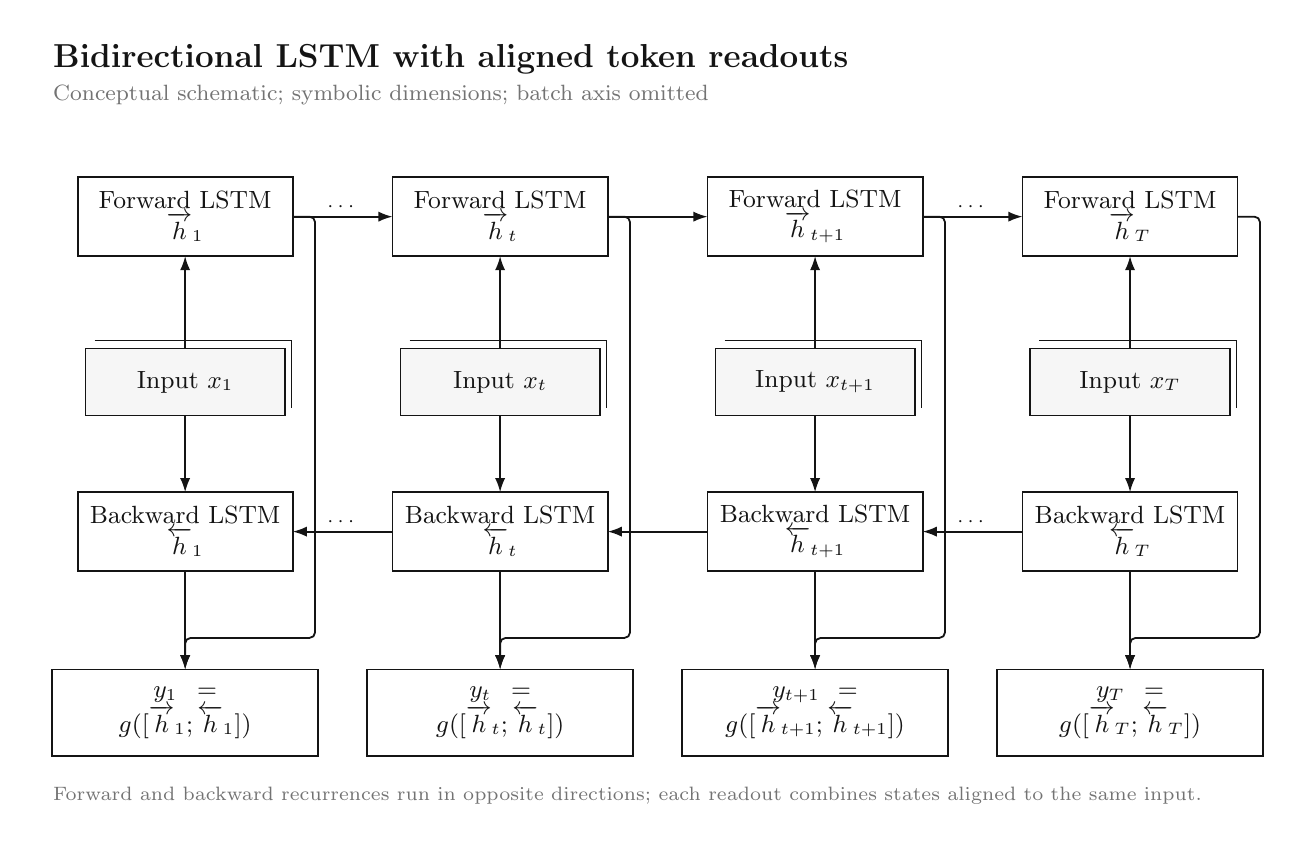
\begin{tikzpicture}[x=1cm,y=-1cm,font=\rmfamily,text=ink]

\path[use as bounding box] (0,0) rectangle (16,10);
\node[anchor=west,font=\large\bfseries] at (.2,.4) {Bidirectional LSTM with aligned token readouts};
\node[anchor=west,font=\footnotesize,text=soft] at (.2,.85) {Conceptual schematic; symbolic dimensions; batch axis omitted};
\begin{pgfonlayer}{background}
\end{pgfonlayer}
\node[box,minimum width=2.7cm,minimum height=1.0cm,text width=2.45cm] (fa) at (2,2.4) {Forward LSTM\\$\overrightarrow h_{1}$};
\node[box,fill=wash,minimum width=2.5cm,minimum height=0.85cm,text width=2.25cm] (xa) at (2,4.5) {Input $x_{1}$};
\draw[ink,line width=.4pt] (0.85,3.975) -- (3.35,3.975) -- (3.35,4.825);
\node[box,minimum width=2.7cm,minimum height=1.0cm,text width=2.45cm] (ba) at (2,6.4) {Backward LSTM\\$\overleftarrow h_{1}$};
\node[box,minimum width=3.35cm,minimum height=1.1cm,text width=3.1cm] (ya) at (2,8.7) {$y_{1}=$\\$g([\overrightarrow h_{1};\overleftarrow h_{1}])$};
\node[box,minimum width=2.7cm,minimum height=1.0cm,text width=2.45cm] (fb) at (6,2.4) {Forward LSTM\\$\overrightarrow h_{t}$};
\node[box,fill=wash,minimum width=2.5cm,minimum height=0.85cm,text width=2.25cm] (xb) at (6,4.5) {Input $x_{t}$};
\draw[ink,line width=.4pt] (4.85,3.975) -- (7.35,3.975) -- (7.35,4.825);
\node[box,minimum width=2.7cm,minimum height=1.0cm,text width=2.45cm] (bb) at (6,6.4) {Backward LSTM\\$\overleftarrow h_{t}$};
\node[box,minimum width=3.35cm,minimum height=1.1cm,text width=3.1cm] (yb) at (6,8.7) {$y_{t}=$\\$g([\overrightarrow h_{t};\overleftarrow h_{t}])$};
\node[box,minimum width=2.7cm,minimum height=1.0cm,text width=2.45cm] (fc) at (10,2.4) {Forward LSTM\\$\overrightarrow h_{t+1}$};
\node[box,fill=wash,minimum width=2.5cm,minimum height=0.85cm,text width=2.25cm] (xc) at (10,4.5) {Input $x_{t+1}$};
\draw[ink,line width=.4pt] (8.85,3.975) -- (11.35,3.975) -- (11.35,4.825);
\node[box,minimum width=2.7cm,minimum height=1.0cm,text width=2.45cm] (bc) at (10,6.4) {Backward LSTM\\$\overleftarrow h_{t+1}$};
\node[box,minimum width=3.35cm,minimum height=1.1cm,text width=3.1cm] (yc) at (10,8.7) {$y_{t+1}=$\\$g([\overrightarrow h_{t+1};\overleftarrow h_{t+1}])$};
\node[box,minimum width=2.7cm,minimum height=1.0cm,text width=2.45cm] (fd) at (14,2.4) {Forward LSTM\\$\overrightarrow h_{T}$};
\node[box,fill=wash,minimum width=2.5cm,minimum height=0.85cm,text width=2.25cm] (xd) at (14,4.5) {Input $x_{T}$};
\draw[ink,line width=.4pt] (12.85,3.975) -- (15.35,3.975) -- (15.35,4.825);
\node[box,minimum width=2.7cm,minimum height=1.0cm,text width=2.45cm] (bd) at (14,6.4) {Backward LSTM\\$\overleftarrow h_{T}$};
\node[box,minimum width=3.35cm,minimum height=1.1cm,text width=3.1cm] (yd) at (14,8.7) {$y_{T}=$\\$g([\overrightarrow h_{T};\overleftarrow h_{T}])$};
\begin{pgfonlayer}{background}
\draw[flow] (xa.north) -- (fa.south);
\draw[flow] (xa.south) -- (ba.north);
\draw[flow] (ba.south) -- (ya.north);
\draw[flow] (fa.east) -- (3.65,2.4) -- (3.65,7.75) -- (2,7.75) -- (ya.north);
\draw[flow] (xb.north) -- (fb.south);
\draw[flow] (xb.south) -- (bb.north);
\draw[flow] (bb.south) -- (yb.north);
\draw[flow] (fb.east) -- (7.65,2.4) -- (7.65,7.75) -- (6,7.75) -- (yb.north);
\draw[flow] (xc.north) -- (fc.south);
\draw[flow] (xc.south) -- (bc.north);
\draw[flow] (bc.south) -- (yc.north);
\draw[flow] (fc.east) -- (11.65,2.4) -- (11.65,7.75) -- (10,7.75) -- (yc.north);
\draw[flow] (xd.north) -- (fd.south);
\draw[flow] (xd.south) -- (bd.north);
\draw[flow] (bd.south) -- (yd.north);
\draw[flow] (fd.east) -- (15.65,2.4) -- (15.65,7.75) -- (14,7.75) -- (yd.north);
\draw[flow] (fa.east) -- (fb.west) node[midway,above,fill=white,inner sep=1.5pt,font=\scriptsize] {$\cdots$};
\draw[flow] (bb.west) -- (ba.east) node[midway,above,fill=white,inner sep=1.5pt,font=\scriptsize] {$\cdots$};
\draw[flow] (fb.east) -- (fc.west);
\draw[flow] (bc.west) -- (bb.east);
\draw[flow] (fc.east) -- (fd.west) node[midway,above,fill=white,inner sep=1.5pt,font=\scriptsize] {$\cdots$};
\draw[flow] (bd.west) -- (bc.east) node[midway,above,fill=white,inner sep=1.5pt,font=\scriptsize] {$\cdots$};
\end{pgfonlayer}
\node[anchor=west,align=left,font=\scriptsize,text=soft,text width=15.6cm] at (.2,9.75) {Forward and backward recurrences run in opposite directions; each readout combines states aligned to the same input.};
\end{tikzpicture}
\end{document}
